\usetikzlibrary{arrows.meta,calc}
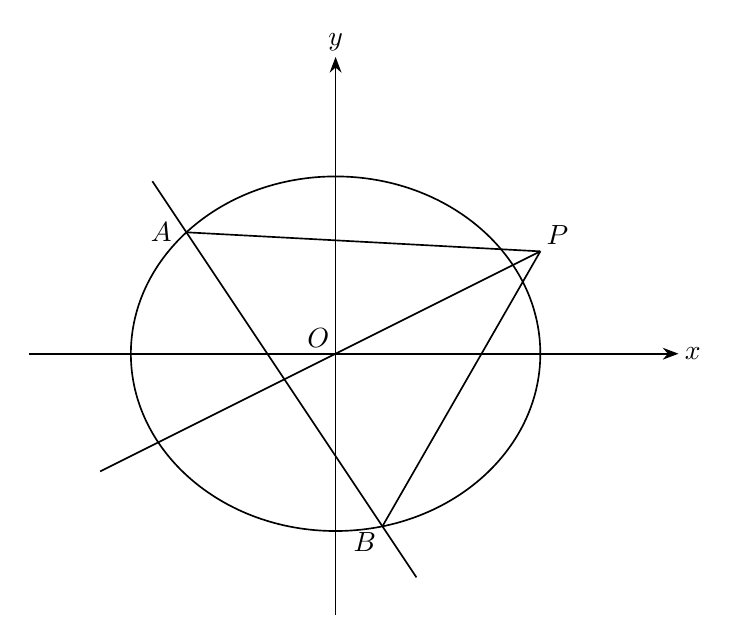
\begin{tikzpicture}[x=1.3cm,y=1.3cm,line width=.6pt,font=\normalsize,>=Stealth,
  label/.style={inner sep=2pt}]
\coordinate (O) at (0,0);
\coordinate (P) at (2,1);
\coordinate (A) at (-1.4574271078,1.1861406616);
\coordinate (B) at (0.4574271078,-1.6861406616);
\coordinate (OPend) at (-2.3,-1.15);
\coordinate (La) at (-1.79,1.685);
\coordinate (Lb) at (0.79,-2.185);
\draw[->] (-3.0,0)--(3.35,0) node[label,right] {$x$};
\draw[->] (0,-2.55)--(0,2.9) node[label,above] {$y$};
\draw (O) ellipse[x radius=2,y radius=1.7320508076];
\draw (La)--(Lb);
\draw (OPend)--(P);
\draw (A)--(P);
\draw (B)--(P);
\node[label,above left] at (O) {$O$};
\node[anchor=east,inner sep=0pt,xshift=-5pt] at (A) {$A$};
\node[label,below left] at (B) {$B$};
\node[label,above right] at (P) {$P$};
\end{tikzpicture}
